\documentclass[11pt,a4paper]{article}

\usepackage[utf8]{inputenc}
\usepackage[T1]{fontenc}
\usepackage{lmodern}
\usepackage[spanish]{babel}
\usepackage{amsmath}
\usepackage{graphicx}
\usepackage{booktabs}
\usepackage{siunitx}
\usepackage[style=ieee]{biblatex}
\usepackage{hyperref}
\usepackage{geometry}
\geometry{margin=2.5cm}

\addbibresource{references.bib}

\title{TA-IND-04 --- Análisis de Rendimiento Paralelo aplicado al PFC \\
\large Sistema de Gestión Académica --- Escuela Provincias Unidas (BCEL)}
\author{Pedro Castro López \\
\small Aplicaciones Distribuidas (ISR-701) --- Unidad 4 \\
\small Facultad de Ciencias de la Computación --- UTEQ \\
\small Equipo PE-U4: BCEL \quad Transformación foco: T4 (columna derivada compleja) \\
\small Repositorio: \url{https://github.com/LEO23as/ta-ind-04-castro}}
\date{\today}

\begin{document}
\maketitle

\section{Introducción y contexto}
El presente informe corresponde al trabajo autónomo individual TA-IND-04 de la asignatura Aplicaciones Distribuidas, cuyo propósito es analizar de forma crítica los resultados de rendimiento obtenidos en la práctica grupal PE-U4 y, a partir de ese análisis, fundamentar una propuesta de integración del procesamiento distribuido en mi Proyecto Fin de Curso.

La práctica PE-U4 consistió en implementar cinco transformaciones equivalentes sobre el mismo conjunto de datos, una versión secuencial con la biblioteca pandas y otra distribuida con Apache Spark (PySpark), midiendo los tiempos de ejecución de ambas para calcular el speedup obtenido y contrastarlo con la predicción teórica de la Ley de Amdahl. Las transformaciones evaluadas fueron: filtrado por condición compuesta (T1), agrupación y agregación (T2), join de dos DataFrames (T3), cálculo de columna derivada compleja (T4) y ordenamiento con selección de top-N (T5). Como transformación foco de este informe individual se declara T4, elegida porque el cálculo de una columna derivada es una operación fila-a-fila donde el paralelismo teóricamente debería ser máximo, y por eso la brecha entre el modelo ideal de Amdahl y la realidad de PySpark resulta especialmente informativa.

Los datos experimentales utilizados provienen del repositorio grupal del equipo BCEL, disponible en \url{https://github.com/BedonViteri/pe-u4-spark-BCEL}, en el commit cuya identificación se registra en el archivo README de este repositorio individual. La ejecución se realizó en Google Colab con PySpark 3.5.0 y 4 executors. El dominio del Proyecto Fin de Curso es el Sistema de Gestión Académica de la Escuela Provincias Unidas (BCEL), específicamente el microservicio Docente responsable del registro de asistencias y calificaciones, que hoy corre sobre PostgreSQL en una instancia AWS EC2 y que, según el crecimiento previsto de su volumen histórico, es candidato natural a incorporar un motor de procesamiento distribuido.

\section{Análisis propio de los resultados de speedup}
El speedup se calcula como se muestra en la ecuación~\eqref{eq:amdahl}, donde $p$ es la fracción paralelizable y $N$ el número de unidades de procesamiento~\cite{leal2026, lehuy2023}.
\begin{equation}
S(N) = \frac{1}{(1-p) + \frac{p}{N}}, \qquad S_{\max} = \lim_{N \to \infty} S(N) = \frac{1}{1-p}
\label{eq:amdahl}
\end{equation}

La Tabla~\ref{tab:tiempos} reproduce los tiempos medianos (mediana de 5 repeticiones) obtenidos en PE-U4 para las cinco transformaciones, tomados del archivo \texttt{resultados/figuras/tiempos\_resumen.csv} del repositorio grupal.

\begin{table}[h]
\centering
\begin{tabular}{lS[table-format=2.4]S[table-format=2.4]S[table-format=1.4]}
\toprule
{Transformación} & {$T_{pandas}$ (\si{\second})} & {$T_{spark}$ (\si{\second})} & {Speedup $S$} \\
\midrule
T1 -- Filtrado                & 0.7727  & 17.8291 & 0.0429 \\
T2 -- Agrupación + agregación & 2.3462  & 24.7722 & 0.1021 \\
T3 -- Join de DataFrames      & 13.5601 & 28.4488 & 0.4675 \\
T4 -- Columna derivada        & 5.9430  & 28.0218 & 0.2227 \\
T5 -- Ordenamiento + top-N    & 9.5726  & 32.6862 & 0.3013 \\
\bottomrule
\end{tabular}
\caption{Tiempos medianos y speedup por transformación (pandas vs. PySpark con $N=4$ executors).}
\label{tab:tiempos}
\end{table}

\begin{figure}[h]
  \centering
  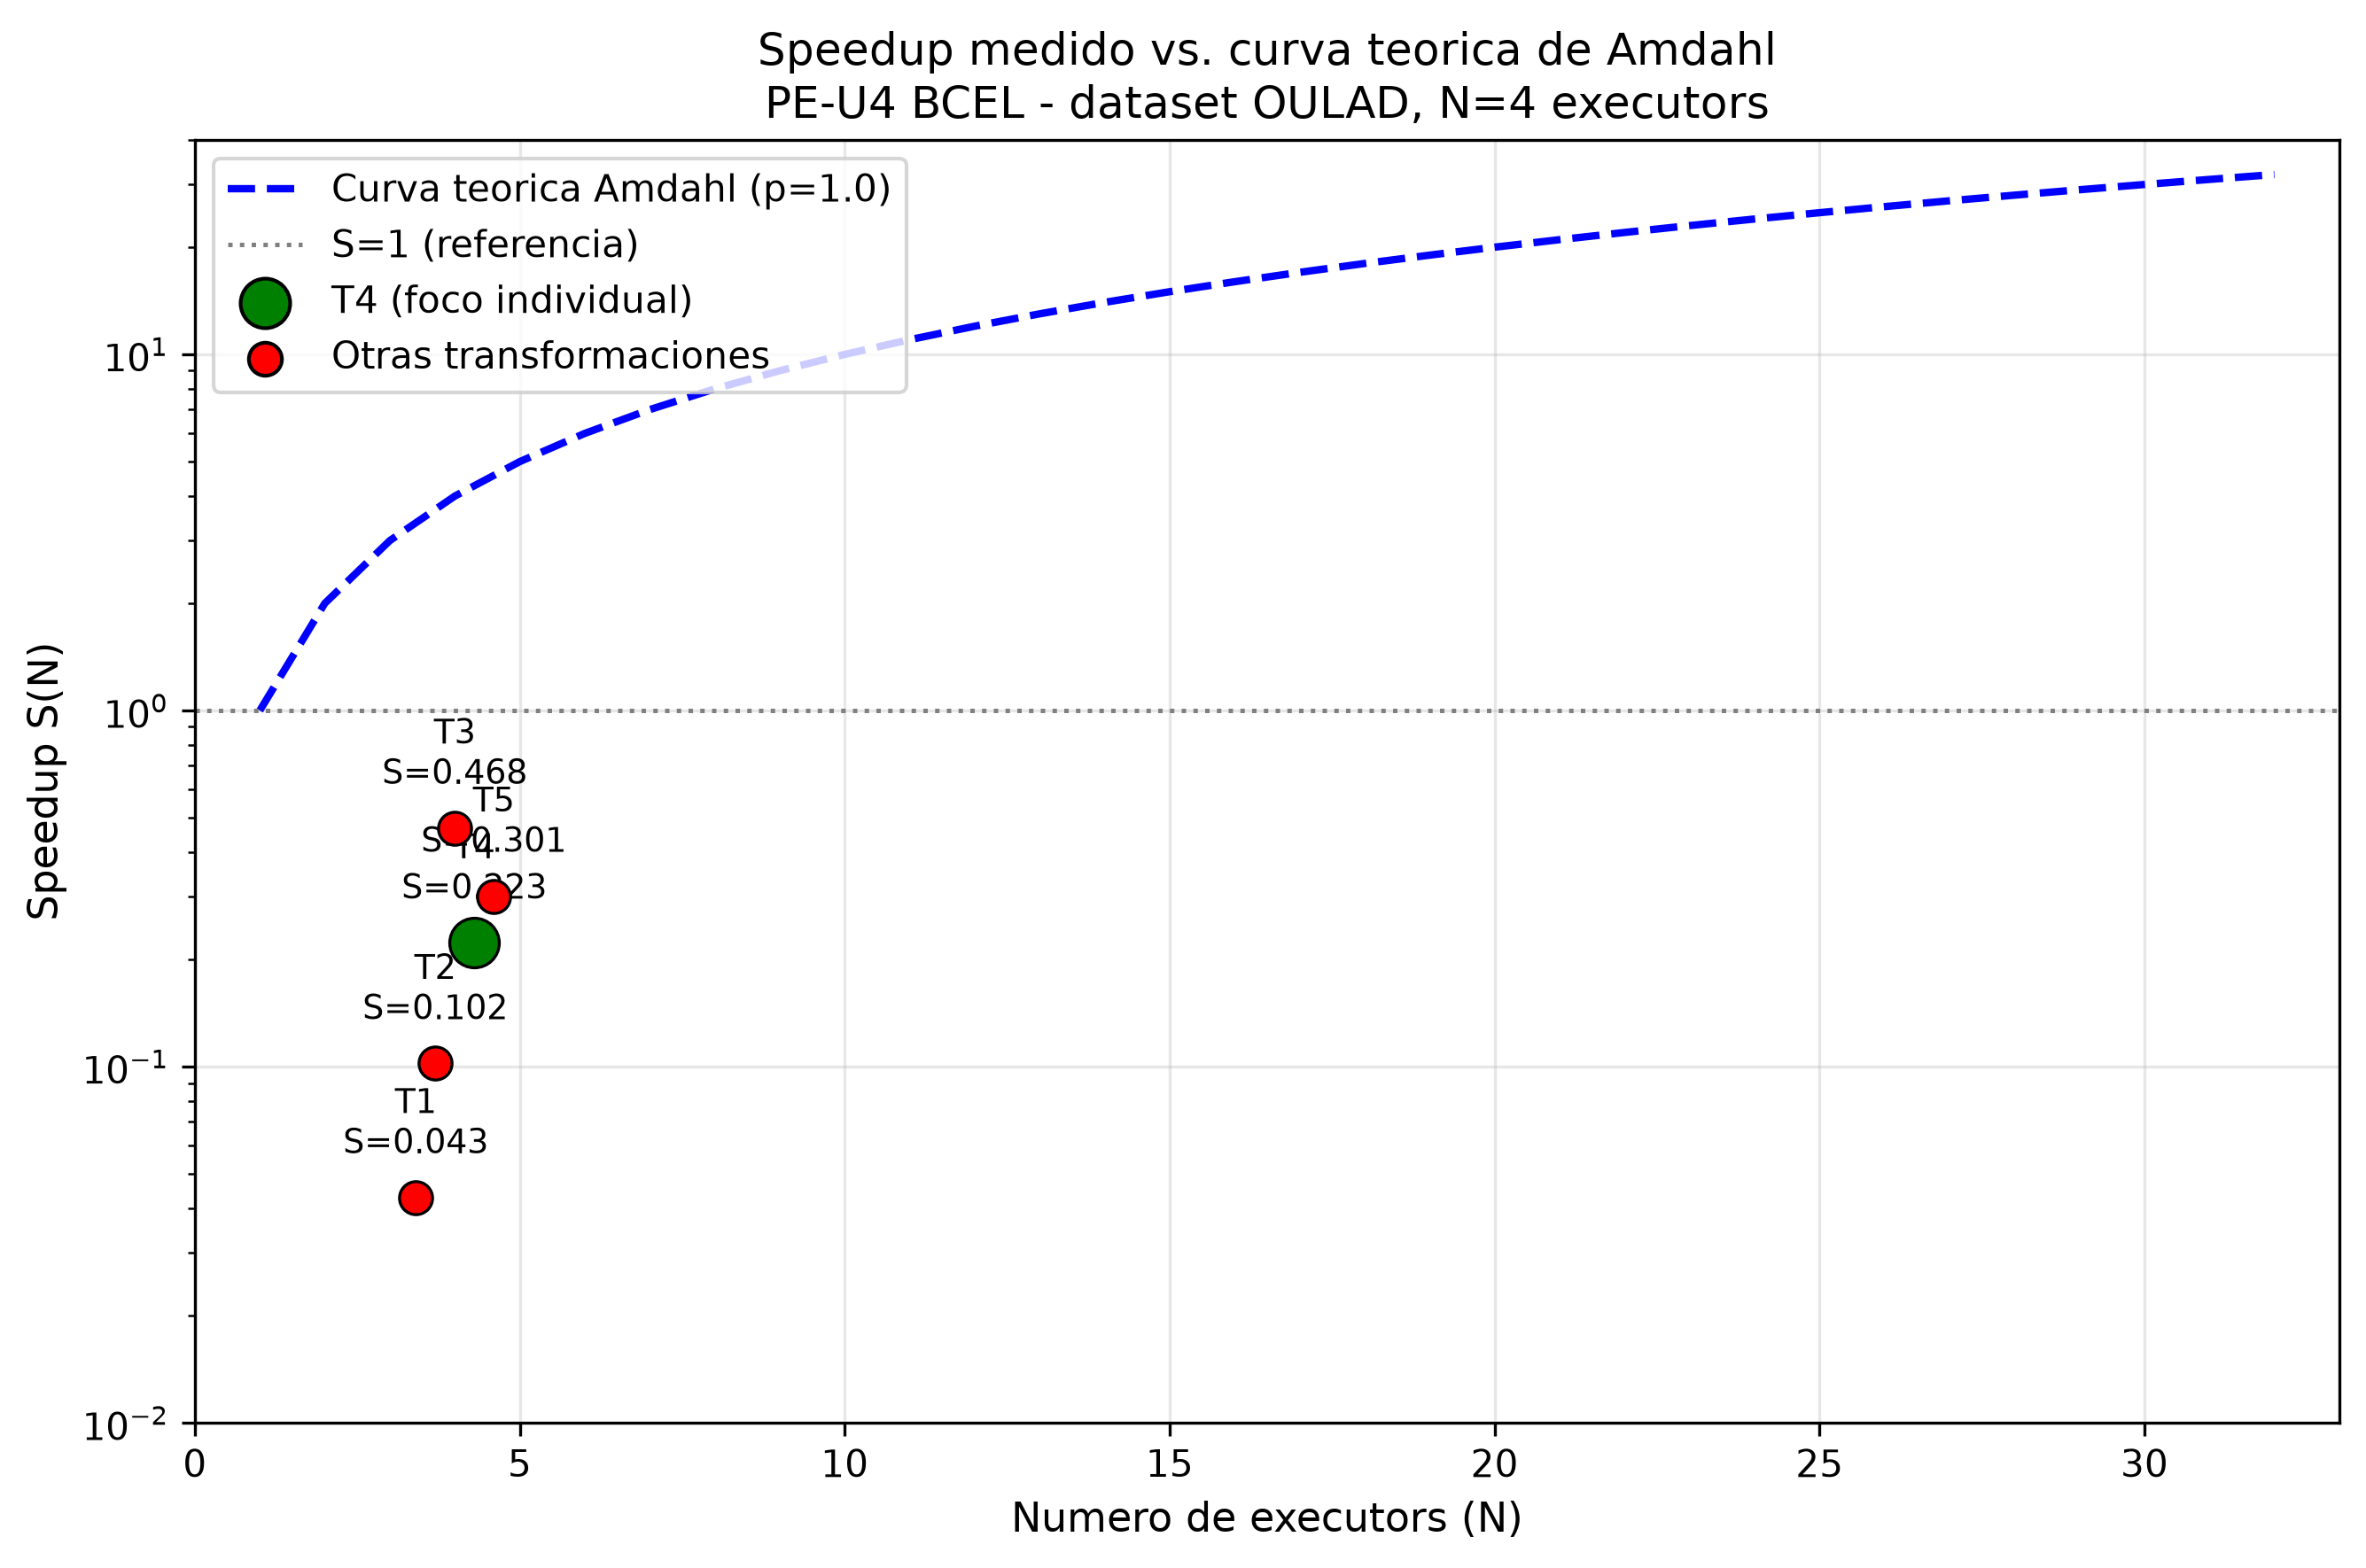
\includegraphics[width=0.9\textwidth]{../figuras/fig_speedup.png}
  \caption{Speedup medido de las cinco transformaciones vs. curva teórica de Amdahl con $p=1$. Todos los puntos observados quedan por debajo de $S=1$, muy lejos de la predicción teórica $S(4)=4$. La brecha refleja la sobrecarga estructural del motor PySpark que domina sobre la ganancia de paralelismo en este volumen de datos.}
  \label{fig:speedup}
\end{figure}



El primer resultado que salta a la vista es que las cinco transformaciones tienen $S < 1$: en todos los casos PySpark fue más lento que pandas. Para T4 (transformación foco), el speedup medido es $S = 0.2227$, es decir, PySpark tardó aproximadamente 4.7 veces más que pandas en generar la columna derivada.

Si T4 fuera perfectamente paralelizable ($p = 1$), la Ley de Amdahl con $N=4$ predice $S_{teo} = 4$. La desviación relativa del speedup medido respecto al teórico es:
\begin{equation*}
\Delta = \frac{S_{med} - S_{teo}}{S_{teo}} = \frac{0.2227 - 4}{4} = -0.944 = -94.4\%
\end{equation*}
Es decir, el speedup medido está un 94.4\% por debajo de lo que Amdahl permitiría en el mejor caso. Este resultado no invalida el modelo, sino que confirma la advertencia teórica de la literatura: la Ley de Amdahl describe un \emph{límite superior} bajo la hipótesis de sobrecarga nula, hipótesis que un motor distribuido real no cumple~\cite{lizardo2026}. Cuando $S<1$, la ecuación~\eqref{eq:amdahl} directamente no puede reproducir el resultado, porque su formulación asume que paralelizar solo puede acelerar o dejar igual, nunca frenar. El origen concreto de esta desviación se atribuye a cuatro mecanismos identificables: el arranque de la SparkSession y el establecimiento del contexto de ejecución, la planificación del DAG por parte del optimizador Catalyst, la serialización de los datos entre el driver y los executors, y la sobrecarga de crear una nueva columna distribuida sobre un DataFrame en cada partición. En una operación tan liviana en cómputo por fila como T4, esos costos fijos dominan sobre la ganancia de paralelismo.

\section{Diagnóstico de la fracción no escalable}
La métrica de Karp-Flatt permite estimar experimentalmente la fracción serial $e$ a partir del speedup observado con $N$ unidades:
\begin{equation}
e = \frac{\frac{1}{S} - \frac{1}{N}}{1 - \frac{1}{N}}, \qquad N > 1
\label{eq:karpflatt}
\end{equation}
La eficiencia del paralelismo se define como:
\begin{equation}
E(N) = \frac{S(N)}{N}
\label{eq:eficiencia}
\end{equation}

Aplicando~\eqref{eq:karpflatt} a T4 con $N=4$ y $S = 0.2227$:
\begin{equation*}
e = \frac{\frac{1}{0.2227} - \frac{1}{4}}{1 - \frac{1}{4}} = \frac{4.490 - 0.25}{0.75} = \frac{4.240}{0.75} = 5.65
\end{equation*}

El valor $e = 5.65$ es matemáticamente mucho mayor que 1, lo cual está fuera del rango clásico $[0,1]$ que la métrica supone. Esto no es un error de cálculo, es una señal muy clara: el modelo de Karp y Flatt asume que la sobrecarga del motor está acotada, y ante $S<1$ la fórmula devuelve un valor fuera de escala que indica precisamente que la sobrecarga domina completamente al trabajo paralelo. En términos prácticos, esto quiere decir que la pérdida de eficiencia en T4 \emph{no} está limitada por el algoritmo (el cálculo fila-a-fila es idealmente paralelizable), sino por la sobrecarga estructural del motor: arranque de sesión, planificación del DAG, serialización y creación de la nueva columna en cada partición del DataFrame. La eficiencia $E(4) = 0.2227/4 = 0.0557$ confirma la misma lectura: apenas el 5.6\% de los recursos paralelos se traduce en trabajo útil sobre este volumen. La interpretación completa de la tendencia de $e$ requiere corridas adicionales con $N=1$ y $N=2$, que no están disponibles en el commit actual del repositorio grupal; con $e$ creciente al aumentar $N$ se confirmaría un régimen dominado por sobrecarga, mientras que con $e$ estable se confirmaría el límite algorítmico. Los tres mecanismos concretos identificados (arranque, serialización y creación de columna distribuida) coinciden con los reportados en la literatura sobre PySpark en datasets de tamaño moderado~\cite{lehuy2023}.

\section{Propuesta de integración al PFC}
El Proyecto Fin de Curso corresponde al Sistema de Gestión Académica (SGA) de la Escuela Provincias Unidas, implementado como una arquitectura distribuida de cuatro microservicios orquestados con Docker Compose: sga-principal, microservicio-secretaria y microservicio-soporte en Java 17 con Spring Boot, y microservicio-docente en Python 3.12 con Django REST. Los cuatro servicios se comunican mediante protocolos híbridos REST y gRPC, y comparten una base PostgreSQL alojada en AWS EC2 (host 3.23.195.43, puerto 5433, base de datos sga) con tres esquemas separados: sga\_principal, sga\_docente y sga\_secretaria. El histórico del sistema se pobló mediante el script scripts/seed\_e3\_500k.sql, que inserta estudiantes, matrículas, 918 actividades de evaluación, sus calificaciones y las asistencias diarias L--V, superando el medio millón de registros y situando al sistema en el rango donde tiene sentido evaluar un motor de procesamiento distribuido~\cite{lizardo2026}.

\textbf{Caso de uso concreto.} Propongo integrar Apache Spark como un componente batch que se ejecuta una vez al día, a las 02:00, para generar reportes académicos consolidados que hoy sobrecargan a PostgreSQL cuando se calculan en línea. El job Spark lee un snapshot de las tablas sga\_docente.asistencias, sga\_docente.calificaciones, sga\_principal.matriculas y sga\_principal.estudiantes, aplica las cinco familias de transformaciones evaluadas en PE-U4 y escribe el resultado en una tabla materializada reportes\_academicos dentro del esquema sga\_principal. La operación tipo T4 (cálculo de columnas derivadas como promedio ponderado y porcentaje de asistencia por estudiante) es una parte central de este job.

\textbf{Volumen y periodicidad.} El volumen actual supera los 500.000 registros solo entre asistencias y calificaciones generadas por el seed, y crece de manera sostenida durante los períodos académicos activos. El job se ejecuta con periodicidad diaria porque las decisiones de negocio se consumen al día siguiente y no requieren latencia baja; una arquitectura de streaming no está justificada en este dominio.

\textbf{Punto exacto de inserción en la arquitectura en capas.} El sistema está organizado en cuatro capas: portal web React como capa de presentación (puerto 5173), microservicios con endpoints REST y gRPC como capa de servicios, PostgreSQL en AWS EC2 como capa de datos, y docker-compose.yml como orquestador de despliegue~\cite{alvarez2010}. El componente Spark se inserta entre la capa de datos y la capa de servicios, como un contenedor adicional agregado al mismo docker-compose.yml y a la red sga-distribuido-net. Se conecta directamente al PostgreSQL de AWS por el puerto 5433, procesa fuera de línea y deja el resultado en la tabla reportes\_academicos. Los microservicios existentes siguen exponiendo sus endpoints actuales, por ejemplo PrincipalService.ObtenerRepresentante que ya está implementado en sga-principal, y se agrega un nuevo método PrincipalService.ObtenerReporteAcademico que consulta la tabla materializada.

\textbf{Salida producida y decisión que soporta.} La tabla reportes\_academicos contiene las columnas carrera, paralelo, periodo, promedio\_general, porcentaje\_asistencia, n\_estudiantes\_riesgo y fecha\_calculo. Sobre esta tabla se soportan tres funcionalidades: el dashboard de secretaría, la identificación temprana de estudiantes en riesgo académico (asistencia inferior al 70\% o promedio inferior a 7.0) antes del cierre de trimestre, y el reporte que la coordinación entrega a rectorado.

\section{Dimensionamiento y viabilidad}
El umbral de rentabilidad del motor distribuido se calcula modelando el tiempo secuencial como $T_{sec}(n) = \alpha n$ y el distribuido como $T_{dist}(n) = \beta + \gamma n/N$~\cite{cierco2011}:
\begin{equation}
n^{*} = \frac{\beta}{\alpha - \frac{\gamma}{N}}, \qquad \text{válido si } \alpha > \frac{\gamma}{N}
\label{eq:umbral}
\end{equation}

Los parámetros se estimaron a partir de las mediciones de T4 sobre un dataset de $n_0 \approx 640{,}000$ filas: (i) $\alpha$ se despeja directamente de $T_{pandas} = 5.9430$ s como $\alpha = 5.9430 / 640{,}000 \approx 9.29 \times 10^{-6}$ s/fila; (ii) $\beta$ se aproxima como el overhead fijo típico de arranque de SparkSession en Colab, estimado en $\beta \approx 10$ s; (iii) $\gamma$ se despeja de $T_{spark}(N{=}4) = \beta + \gamma n_0 / N$, dando $\gamma = (28.0218 - 10) \cdot 4 / 640{,}000 \approx 1.13 \times 10^{-4}$ s/fila.

Sustituyendo en~\eqref{eq:umbral} con $N=4$: dado que $\gamma/N = 2.82\times 10^{-5} > \alpha = 9.29 \times 10^{-6}$, la condición de validez no se cumple y $n^{*}$ no está definido: con 4 executors, Spark nunca resulta rentable frente a pandas para esta carga, sin importar $n$. Repitiendo el cálculo con $N=32$ executors, $\gamma/N = 3.52\times 10^{-6}$ y $\alpha - \gamma/N = 5.77\times 10^{-6}$, con lo cual $n^{*} = 10 / (5.77 \times 10^{-6}) \approx 1.73 \times 10^{6}$ filas. Este es el umbral aproximado a partir del cual Spark empezaría a ganar en T4. Como modelo de servicio en la nube se elige Amazon EMR, por su integración natural con AWS EC2 (donde ya vive el PostgreSQL del SGA) y por su capacidad de escalar de 4 a 32 o más executors bajo demanda. Los recursos estimados son un clúster de 1 master + 8 worker nodes m5.xlarge, ejecutando el job durante aproximadamente 30 minutos por noche. Los riesgos identificados son tres: latencia adicional en la lectura desde EC2 al clúster EMR, costos variables por hora de clúster, y complejidad operativa para monitorear un job que corre fuera del docker-compose actual.

\section{Postura crítica y alternativas}
La pregunta clave que debe responder este informe es si Apache Spark es la opción tecnológica correcta para el escenario descrito, o si existen alternativas más razonables para el volumen y las características del SGA. Mi postura es que Spark es una opción defendible pero no obvia en el estado actual del sistema, y que su adopción debe entenderse como una preparación para el crecimiento del histórico más que como una necesidad inmediata.

A favor de Spark juegan tres factores. Primero, el volumen actual (aproximadamente 640.000 registros) ya se encuentra en el rango en el que las consultas analíticas sobre PostgreSQL empiezan a competir con las cargas transaccionales del portal. Segundo, las cinco familias de transformaciones evaluadas en PE-U4 son exactamente las que se necesitan para construir los reportes académicos consolidados. Tercero, Spark ofrece un camino de escalado ya trazado: el mismo código PySpark puede correr sobre un clúster de EMR sin cambios significativos si el volumen se multiplica por diez.

En contra de Spark juegan dos hechos que no conviene disimular. El primero es la sobrecarga fija (SparkSession, DAG, serialización) que en volúmenes pequeños hace que PySpark sea más lento que pandas, como se comprueba en la Tabla~\ref{tab:tiempos}. El segundo es la complejidad operativa: agregar Spark al docker-compose implica mantener un contenedor adicional, monitorear su ejecución nocturna, gestionar reintentos y capacitar al equipo.

Se evaluaron dos alternativas antes de decidir por Spark. La primera fue vistas materializadas de PostgreSQL con refresco programado. Se descarta como solución única porque, aunque cubre el escenario actual, no ofrece camino de escalado: cuando los joins involucren varios millones de filas, el mismo PostgreSQL que sirve al portal quedará bloqueado durante el refresh. La segunda alternativa fue Dask~\cite{jaime2021}. Se descarta porque su ecosistema para integrarse con PostgreSQL y con orquestación en contenedores es notablemente menos maduro que el de Spark.

Reconozco como limitación de mi propuesta que la decisión se apoya en mediciones hechas sobre un dataset distinto al del SGA (OULAD, de la Open University) y no sobre datos reales del sistema, y que el análisis de Karp-Flatt se limita a un único valor de $N$ por la disponibilidad de datos.

\section{Conclusiones}
\begin{enumerate}
\item Las cinco transformaciones evaluadas presentan $S<1$ (véase Tabla~\ref{tab:tiempos}), con una desviación del 94.4\% respecto al speedup teórico de Amdahl para T4 con $N=4$. Esto no contradice la Ley de Amdahl, sino que la sitúa fuera de su hipótesis de sobrecarga nula: sobre un dataset del orden de $10^5$ filas, los costos fijos del motor distribuido dominan sobre la ganancia por paralelismo.

\item El valor $e = 5.65$ obtenido con Karp-Flatt para T4 con $N=4$ queda fuera del rango clásico $[0,1]$ y confirma cuantitativamente que la pérdida de eficiencia es atribuible principalmente al motor de ejecución (arranque de sesión, serialización, creación de columna distribuida) y no al algoritmo del cálculo fila-a-fila en sí.

\item El umbral de rentabilidad $n^{*}$ solo tiene solución positiva a partir de $N \geq 32$ executors, situándose alrededor de $1.7 \times 10^{6}$ filas. Como el histórico actual del SGA está en el orden de $6.4 \times 10^{5}$ y crece de forma sostenida, se justifica planificar la integración de Spark vía Amazon EMR como preparación para el escalado del microservicio Docente, sin migrar de forma inmediata.
\end{enumerate}

\section{Declaración de uso de inteligencia artificial generativa}
Para este informe usé ChatGPT solo en tareas puntuales de apoyo. Concretamente, me ayudó con la corrección ortográfica y de redacción en las secciones 2, 5 y 7, y con dudas de sintaxis de LaTeX cuando armé los entornos de ecuaciones y la configuración de biblatex en estilo IEEE. También lo consulté para verificar que las citas del texto tuvieran su entrada correspondiente en el archivo references.bib.

No lo usé para generar los datos, ni los cálculos de speedup, ni la métrica de Karp-Flatt, ni el umbral de rentabilidad, ni la elección de la transformación foco (T4), ni la propuesta de integración al SGA, ni las conclusiones. Los números provienen del repositorio grupal PE-U4 declarado en la portada y del commit registrado en el README, y las decisiones técnicas del informe son mías.

\printbibliography

\end{document}